\documentclass[11pt,a4paper]{extarticle}

\usepackage[a4paper, top=2cm, bottom=2cm, left=2.2cm, right=2.2cm]{geometry}
\usepackage[utf8]{inputenc}
\usepackage[T1]{fontenc}
\usepackage{lmodern}

\usepackage{booktabs}
\usepackage{tabularx}
\usepackage{graphicx}
\usepackage{float}
\usepackage{parskip}
\usepackage{enumitem}
\usepackage{titlesec}
\usepackage{hyperref}
\usepackage{xcolor}
\usepackage{fancyvrb}
\usepackage{amsmath}

% Tighter section spacing to save space
\titlespacing{\section}{0pt}{0.9em}{0.4em}
\titlespacing{\subsection}{0pt}{0.7em}{0.25em}

% Tighter list spacing
\setlist[itemize]{itemsep=1pt, topsep=3pt, parsep=0pt}
\setlist[enumerate]{itemsep=1pt, topsep=3pt, parsep=0pt}

\hypersetup{colorlinks=true, linkcolor=black, urlcolor=blue}

% ---------------------------------------------------------------
\begin{document}
\sloppy

% ── Title block ─────────────────────────────────────────────────
\begin{center}
  {\LARGE\bfseries Assignment 2: Text Processing and Classification using Apache Spark}\\[0.6em]
\end{center}

\vspace{0.4em}
\noindent\textbf{Contributors:}
Hassan Ali \quad Odedra Mayurbhai Jakharabhai \quad Petho Dominik \quad Robea Anda-Teodora \quad Rusu Paisie
\vspace{0.3em}\hrule\vspace{0.5em}

% ── 1. Introduction ─────────────────────────────────────────────
\section{Introduction}

This assignment extends Assignment 1's single-node chi-square text pipeline to Apache Spark across three parts. The first part reproduces the chi-square term ranking using the low-level RDD API. Second builds a Spark ML TF-IDF feature extraction pipeline and third, extends that pipeline with a multi-class SVM classifier tuned via 24-combination grid search.

% ── 2. Problem Overview ─────────────────────────────────────────
\section{Problem Overview}

The Amazon Review Dataset (\texttt{reviews\_devset.json}) contains reviews across 22 product categories, each with a \texttt{reviewText} field and a \texttt{category} label.

\begin{itemize}
  \item \textbf{Part 1:} Compute per-category chi-square scores, select top-75 terms per category, write \texttt{output\_rdd.txt} matching Assignment 1's format.
  \item \textbf{Part 2:} Build a Spark ML \texttt{Pipeline} (tokenise $\to$ TF-IDF $\to$ chi-square selection, top 2000 globally) and write \texttt{output\_ds.txt}.
  \item \textbf{Part 3:} Extend Part 2 with L2 normalisation and \texttt{OneVsRest(LinearSVC)}, run grid search, evaluate weighted F1 on a held-out test set.
\end{itemize}

% ── 3. Methodology ──────────────────────────────────────────────
\section{Methodology and Approach}

\begin{figure}[htbp]
\centering
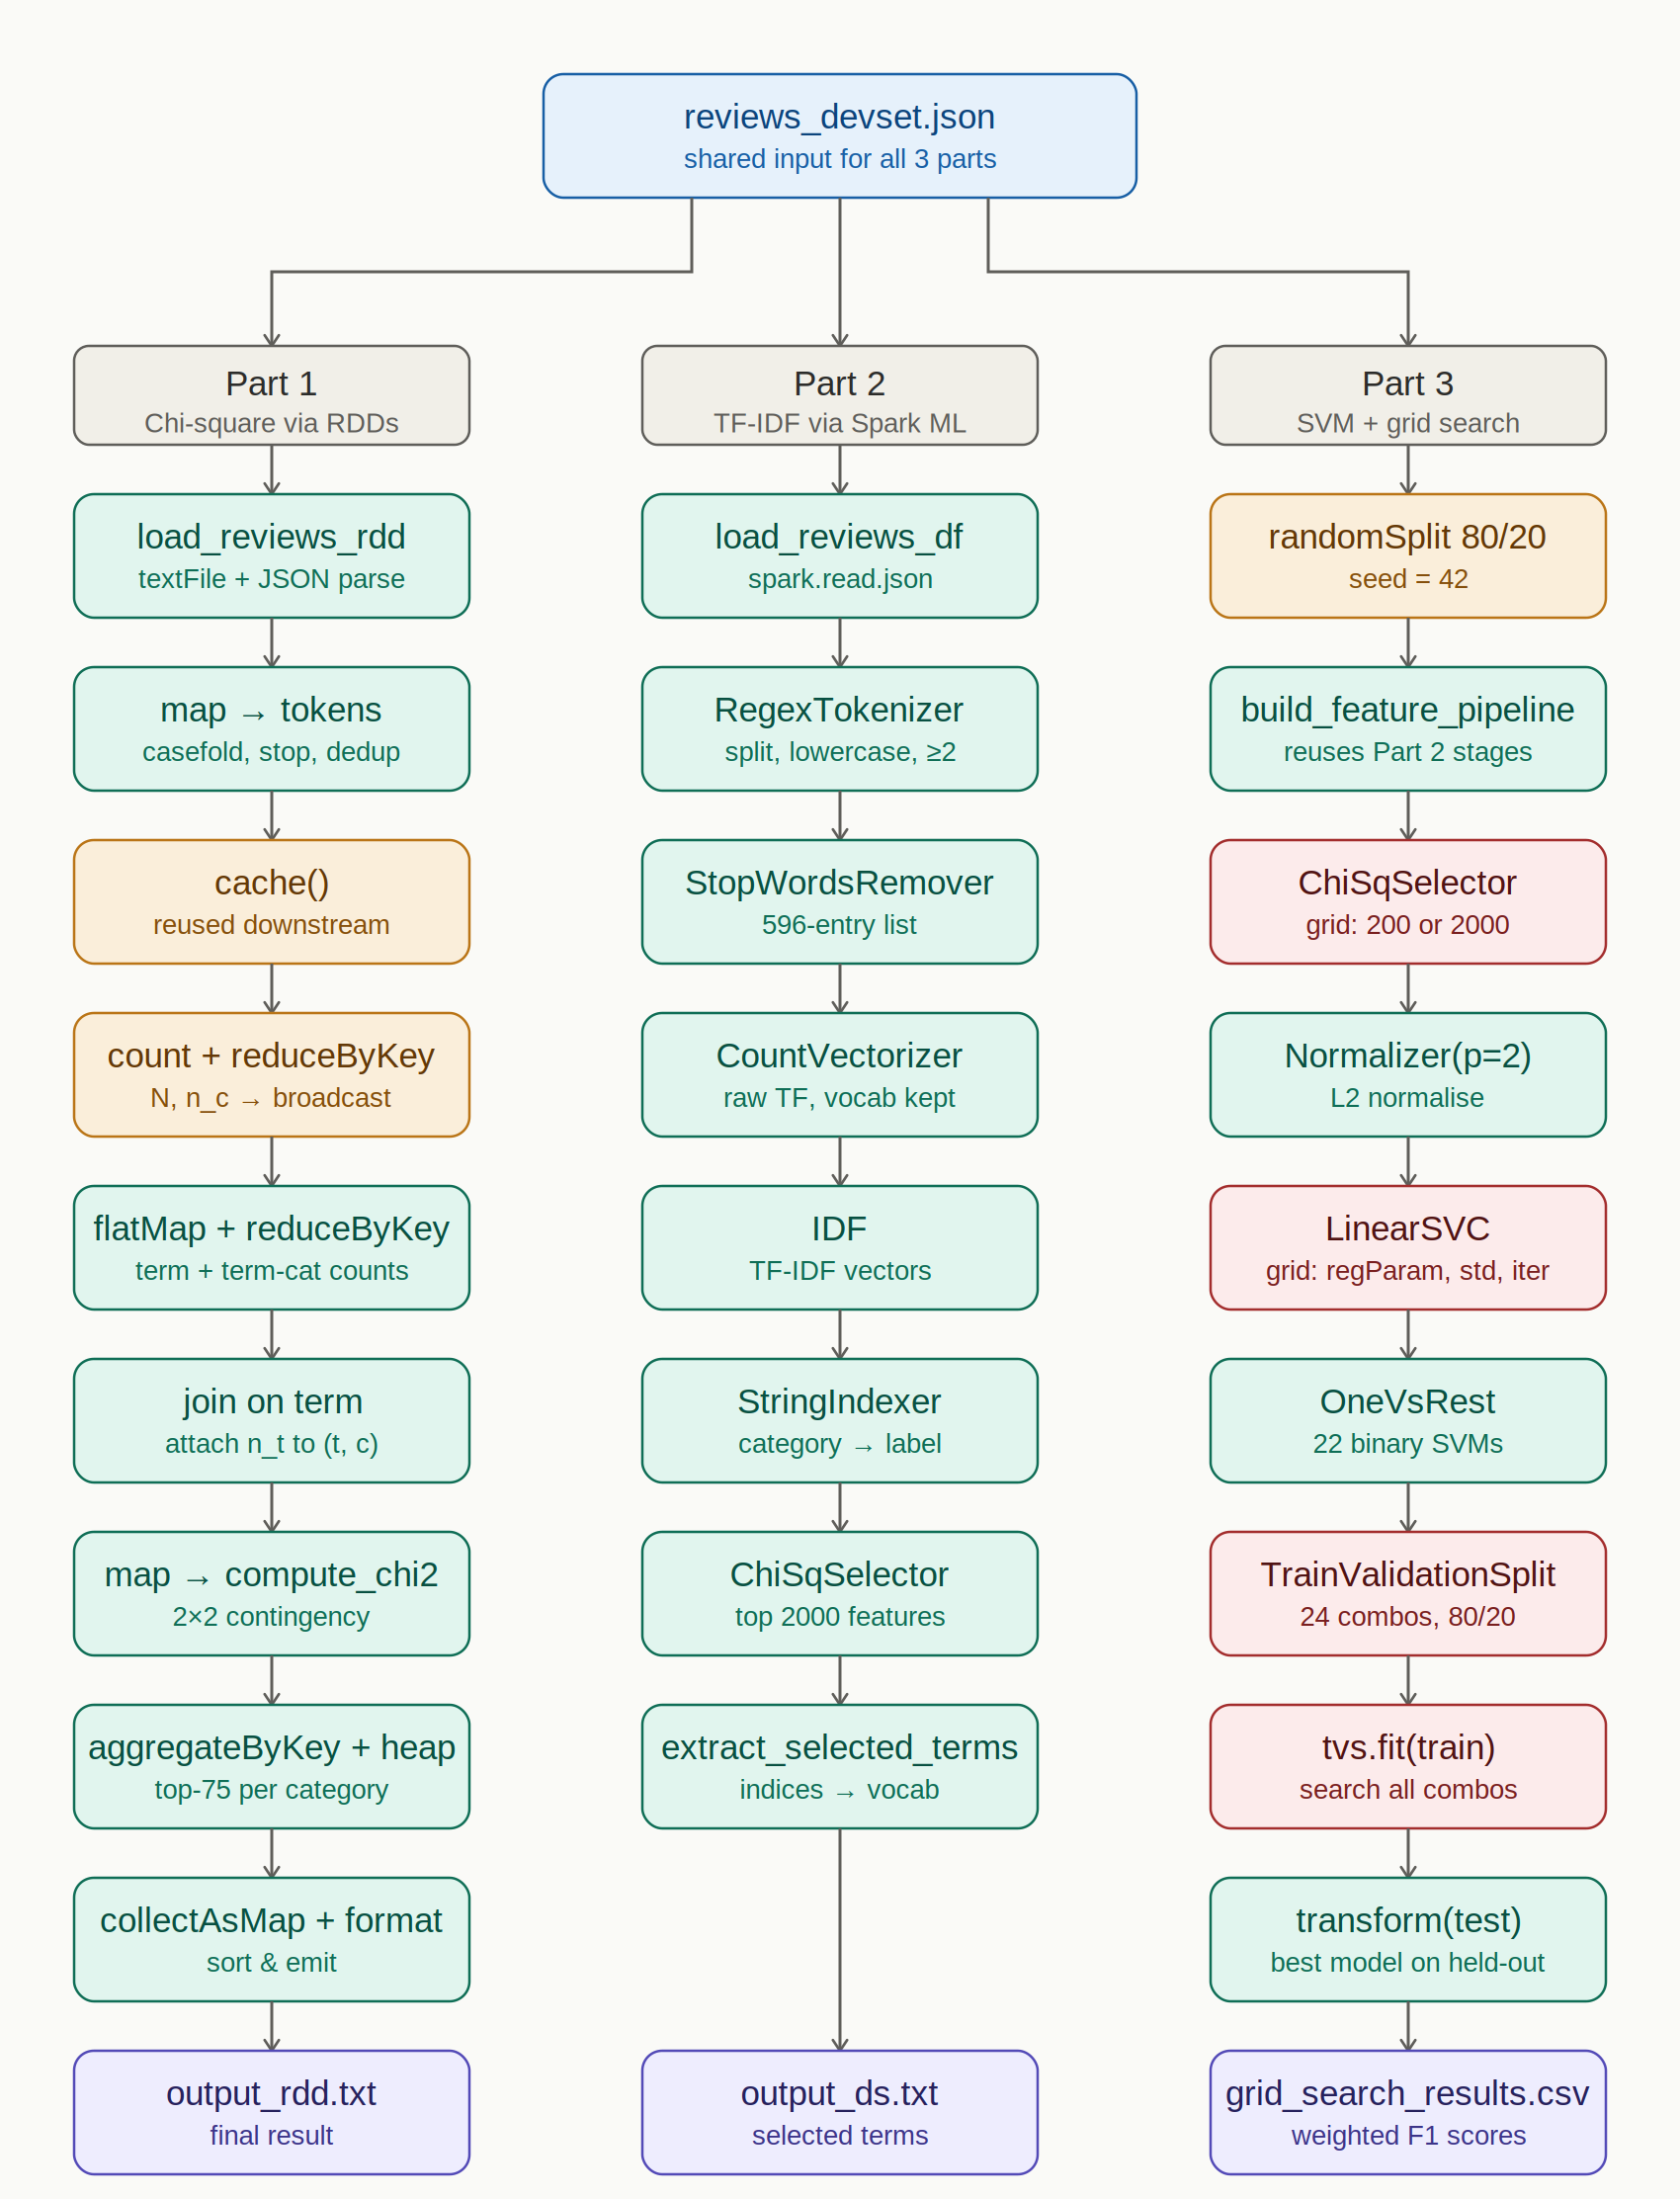
\includegraphics[width=0.55\linewidth]{combined_pipeline.png}
\caption{Combined pipeline}
\label{fig:part3}
\end{figure}

\subsection{Shared Preprocessing (\texttt{src/common/})}

To ensure consistent text handling across the pipeline, all three parts of the implementation rely on a single tokenisation module, \texttt{text\_utils.py}. Text is split on whitespace, digits, and delimiters \texttt{()[]\{\}.!?,;:+=-\_"'\textasciitilde\#@\&*\%€\$§\/}, casefolded, and tokens shorter than 2 characters are discarded. A uniform stopword filter containing 596 entries is then applied. Because the pipeline executes in two distinct environments, the underlying regular expression is maintained in two equivalent forms: a native Python pattern, \texttt{TOKEN\_SPLIT\_RE}, used in Part 1, and \texttt{REGEX\_TOKENIZER\_PATTERN}, which is consumed by Spark ML's \texttt{RegexTokenizer} in Parts 2 and 3.

% ─── Part 1 ──────────────────────────────────────────────────
\subsection{Part 1 — Chi-Square via Spark RDDs}

\textbf{Processing steps:}
\begin{enumerate}
  \item The JSON review file is ingested into an RDD through the helper \texttt{load\_reviews\_rdd()}.
  \item Each record is then mapped to the form \texttt{(category, deduped\_tokens)}. Deduplication is performed at the document level so that the chi-square statistic reflects term \emph{presence} rather than raw frequency.
  \item The resulting \texttt{(category, tokens)} RDD is \textbf{cached} in memory to prevent the input data from being read more than once.
  \item Both $N$ and $n_c$ are computed with \texttt{reduceByKey} and subsequently \textbf{broadcast} to all executors.
  \item A single \texttt{flatMap} stage emits the tagged keys \texttt{("T",~term)} and \texttt{("TC",~term,~cat)}, which are then consolidated by a single \texttt{reduceByKey}; this design produces both $n_t$ and $n_{tc}$ within one shuffle.
  \item A \texttt{join} on the term key attaches $n_t$ to every \texttt{(term,~cat)} pair.
  \item Each pair is passed through \texttt{compute\_chi2()}, which applies the standard $2{\times}2$ contingency formula.
  \item To avoid the cost of \texttt{groupByKey}, the top-$K$ terms per category are selected using \texttt{aggregateByKey} together with a bounded min-heap of size 75.
  \item Finally, \texttt{collectAsMap} retrieves the small result table ($22{\times}75$ rows), which is formatted and persisted as \texttt{output\_rdd.txt}.
\end{enumerate}
\vspace{0.4em}

\textbf{Key functions:}
\begin{itemize}
  \item \texttt{compute\_chi2(N, n\_t, n\_c, n\_tc)} implements the standard $2{\times}2$ contingency chi-square test and returns \texttt{None} whenever the denominator evaluates to zero.
  \item \texttt{\_make\_heap\_ops(top\_k)} produces the \texttt{seq\_op} and \texttt{comb\_op} closures required by \texttt{aggregateByKey}. Each partition maintains a min-heap bounded to \texttt{top\_k} entries, with the weakest term evicted whenever the heap exceeds its capacity.
  \item \texttt{\_RevStr} a thin string wrapper that inverts the natural ordering so that, on chi-square ties, alphabetically larger terms are evicted first, in line with the tie-breaking convention defined in Assignment 1.
  \item \texttt{format\_output(result)} --- orders the terms within each category by $(-\chi^2,\ \mathrm{term})$ and appends, as the final line, the alphabetically sorted union of all surviving terms.
  \item \texttt{run(...)} coordinates the full RDD pipeline by initialising the Spark context, broadcasting the stopword list and $n_c$, chaining the transformations described above, and writing the output file.
\end{itemize}

% ─── Part 2 ──────────────────────────────────────────────────
\subsection{Part 2 - TF-IDF Pipeline via Spark ML}

\textbf{Processing steps:}

\begin{enumerate}
    \item The review corpus is first loaded as a DataFrame using \texttt{load\_reviews\_df()}.
    \item The 596-entry stopword list is passed directly from the driver into the pipeline, since the list is small enough that explicit broadcasting offers no measurable benefit.
    \item A six-stage \texttt{Pipeline} is then assembled through the \texttt{build\_feature\_pipeline()} factory function.
    \item The complete pipeline is trained in a single \texttt{.fit(df)} invocation.
    \item Once fitted, the selected term strings are recovered by mapping the indices stored in \texttt{ChiSqSelectorModel.selectedFeatures} back onto the vocabulary of the \texttt{CountVectorizerModel}.
    \item Finally, the 2000 selected terms are sorted alphabetically and written to \texttt{output\_ds.txt}.
\end{enumerate}

\vspace{0.4em}
\textbf{Key functions:}

\begin{itemize}
    \item \texttt{build\_feature\_pipeline(num\_top\_features\, stopwords)} constructs and returns an \emph{unfitted} \texttt{Pipeline}. \texttt{CountVectorizer} is deliberately preferred over \texttt{HashingTF} so that the vocabulary remains recoverable, while \texttt{StringIndexer} produces the numeric category labels required by \texttt{ChiSqSelector}. The same factory is reused without modification in Part 3.
    \item \texttt{extract\_selected\_terms(fitted\_pipeline)} resolves the indices in \texttt{selectedFeatures} against the \texttt{CountVectorizerModel.vocabulary} and returns the resulting terms in alphabetical order.
    \item \texttt{run(...)} coordinates the workflow by invoking the factory, fitting the pipeline once, extracting the selected terms, and writing the output file.
\end{itemize}

% ─── Part 3 ──────────────────────────────────────────────────
\subsection{Part 3 - Multi-Class SVM Classification and Grid Search}

\textbf{Processing steps:}
\begin{enumerate}
  \item The dataset is first partitioned into \texttt{train\_data} and \texttt{test\_data} using an 80/20 split with \texttt{seed=42} to guarantee reproducibility.
  \item The feature pipeline defined in Part 2 is reused through the same \texttt{build\_feature\_pipeline()} factory, avoiding any duplication of preprocessing logic.
  \item An additional \texttt{Normalizer(p=2.0)} stage is appended so that the resulting TF-IDF vectors are L2-normalised prior to classification.
  \item Multi-class support across the 22 product categories is achieved by wrapping \texttt{LinearSVC} inside a \texttt{OneVsRest} meta-classifier.
  \item A parameter grid containing 24 configurations (2$\times$3$\times$2$\times$2) is then constructed to explore the relevant hyperparameter space.
  \item Hyperparameter search is carried out on \texttt{train\_data} using \texttt{TrainValidationSplit(trainRatio=0.8, seed=42)}.
  \item The configuration with the highest validation score is subsequently evaluated on \texttt{test\_data} using \texttt{MulticlassClassificationEvaluator(f1)}.
  \item Finally, the validation F1 score of every one of the 24 grid combinations is persisted to \texttt{grid\_search\_results.csv} for later analysis.
\end{enumerate}

\vspace{0.4em}
\textbf{Grid search space (24 combinations):}

\begin{center}
\begin{tabular}{ll}
\toprule
\textbf{Parameter} & \textbf{Values} \\
\midrule
\texttt{numTopFeatures} & 200, 2000 \\
\texttt{regParam}       & 0.01, 0.1, 1.0 \\
\texttt{standardization}& True, False \\
\texttt{maxIter}        & 10, 50 \\
\bottomrule
\end{tabular}
\end{center}

\vspace{0.4em}
\textbf{Key functions:}

\begin{itemize}
  \item \texttt{build\_spark(mode)} --- initialises the \texttt{SparkSession}; under local execution the driver is pinned to \texttt{127.0.0.1}, whereas in cluster mode the master assignment is delegated to YARN.
  \item \texttt{run(...)} --- orchestrates the end-to-end workflow by assembling the full pipeline, constructing the parameter grid, running \texttt{TrainValidationSplit}, evaluating the best model on the held-out test set, and persisting the grid search results as a CSV file.
\end{itemize}


% ── 4. Results ──────────────────────────────────────────────────
\section{Results}

\subsection{Part 1 - RDD Output vs.\ Assignment 1}

\begin{center}
\begin{tabular}{lc}
\toprule
\textbf{Category} & \textbf{Overlap} \\
\midrule
Apps\_for\_Android            & 66/75 \\
Automotive                    & 49/75 \\
Baby                          & 57/75 \\
Beauty                        & 65/75 \\
Books                         & 70/75 \\
CDs\_and\_Vinyl               & 71/75 \\
Cell\_Phones\_and\_Accessories & 66/75 \\
Clothing\_Shoes\_and\_Jewelry & 70/75 \\
Digital\_Music                & 46/75 \\
Electronics                   & 72/75 \\
Grocery\_and\_Gourmet\_Food   & 65/75 \\
Health\_and\_Personal\_Care   & 60/75 \\
Home\_and\_Kitchen            & 63/75 \\
Kindle\_Store                 & 59/75 \\
Movies\_and\_TV               & 66/75 \\
Musical\_Instruments          & 48/75 \\
Office\_Products              & 54/75 \\
Patio\_Lawn\_and\_Garden      & 55/75 \\
Pet\_Supplies                 & 56/75 \\
Sports\_and\_Outdoors         & 59/75 \\
Tools\_and\_Home\_Improvement & 60/75 \\
Toys\_and\_Games              & 61/75 \\
\textbf{Average}              & \textbf{60.8/75 (81.1\%)} \\
\bottomrule
\end{tabular}
\end{center}

\vspace{0.5em}
After merging the per-category dictionaries, the RDD implementation produces 1{,}464 terms compared with 1{,}418 terms in Assignment~1, of which \textbf{1{,}177 (83.0\%)} are shared by both. The remaining divergence is attributable to two factors. First, the order in which partial sums are combined inside Spark's distributed \texttt{reduceByKey} is non-deterministic, which introduces small floating-point variations across executors. Second, subtle differences in Unicode handling between Python's \texttt{casefold()} and Java's \texttt{toLowerCase()} occasionally produce distinct surface forms for the same input. The three categories with the lowest overlap (Digital\_Music with 46, Musical\_Instruments with 48, and Automotive with 49) are precisely those in which a large number of terms cluster around very similar chi-square values, so that minute numerical perturbations are sufficient to flip the rank at the cut-off boundary.


\subsection{Part 2 - DataFrame Pipeline vs.\ Assignment 1}
\begin{center}
\begin{tabular}{ll}
\toprule
\textbf{Metric} & \textbf{Value} \\
\midrule
Part 2 selected terms (\texttt{output\_ds.txt}) & 2,000 \\
Assignment 1 merged dictionary                  & 1,418 \\
Terms in both                                   & 763 \\(53.8\% of Asgn.\ 1) \\
Only in Part 2                                  & 1,237 \\
Only in Assignment 1                            & 655 \\
\bottomrule
\end{tabular}
\end{center}

The two selection strategies clearly target different parts of the term distribution. The 1{,}237 terms unique to Part 2 are typically mid-frequency vocabulary items that achieve high TF-IDF chi-square scores at the global level without being strongly tied to any single category. Conversely, the 655 terms absent from Part 2 are predominantly category-specific jargon (e.g.\ \textit{ableton}, \textit{airsoft}); such terms rank within the per-category top-75 of Assignment 1 but fall outside the global top 2{,}000 selected by the DataFrame pipeline.


\subsection{Part 3 - SVM and Grid Search Results}
\begin{table}[htbp]
\centering
\caption{All 24 combinations sorted by validation F1}
\label{tab:gs}
\small
\begin{tabular}{ccccc c}
\toprule
\textbf{Rank} & \textbf{numTopFeat.} & \textbf{regParam} & \textbf{std.} & \textbf{maxIter} & \textbf{Val.\ F1} \\
\midrule
1 & 2000 & 0.01 & T & 10 & \textbf{0.6077} \\
2 & 2000 & 0.01 & T & 50 & 0.6030 \\
3 & 2000 & 0.10 & T & 10 & 0.6021 \\
4 & 2000 & 0.10 & T & 50 & 0.5938 \\
5 & 2000 & 1.00 & T & 10 & 0.5708 \\
6 & 2000 & 1.00 & T & 50 & 0.5526 \\
7 & 2000 & 0.10 & F & 50 & 0.4993 \\
8 & 2000 & 0.01 & F & 50 & 0.4980 \\
9 & 200  & 0.01 & T & 10 & 0.3817 \\
10 & 200  & 0.10 & T & 10 & 0.3719 \\
11 & 200  & 0.01 & T & 50 & 0.3710 \\
12 & 200  & 0.10 & T & 50 & 0.3583 \\
13 & 2000 & 0.01 & F & 10 & 0.3563 \\
14 & 200  & 1.00 & T & 10 & 0.3376 \\
15 & 200  & 0.01 & F & 50 & 0.3317 \\
16 & 200  & 1.00 & T & 50 & 0.3303 \\
17 & 200  & 0.10 & F & 50 & 0.3260 \\
18 & 200  & 0.01 & F & 10 & 0.3258 \\
19 & 200  & 1.00 & F & 50 & 0.3244 \\
20 & 200  & 0.10 & F & 10 & 0.2696 \\
21 & 2000 & 1.00 & F & 10 & 0.1241 \\
22 & 2000 & 0.10 & F & 10 & 0.1240 \\
23 & 200  & 1.00 & F & 10 & 0.0008 \\
24 & 2000 & 1.00 & F & 50 & 0.0005 \\
\bottomrule
\end{tabular}
\end{table}

\textbf{Best model test-set F1: 0.6077} (numTopFeatures=2000, regParam=0.01, standardization=True, maxIter=10).
Among the four hyperparameters examined, \textbf{feature dimensionality} emerges as the dominant factor: every one of the top eight configurations uses 2{,}000 features, with F1 scores ranging from 0.499 to 0.608, whereas the best 200-feature configuration plateaus at 0.382, a drop of roughly 0.22 points. \textbf{Standardisation} proves to be effectively mandatory; when it is disabled in combination with \texttt{regParam}=1.0, the F1 score collapses to near zero, since the widely varying scales of the TF-IDF features destabilise the gradient updates. \textbf{Regularisation strength} also exhibits a consistent trend when standardisation is enabled: smaller values of \texttt{regParam} (0.01) outperform larger ones. Finally, the \textbf{maximum number of iterations} exerts only a modest influence; \texttt{maxIter}=10 frequently matches or even surpasses \texttt{maxIter}=50, which indicates that the optimiser converges rapidly on L2-normalised TF-IDF features.





% ── 5. Conclusions ──────────────────────────────────────────────
\section{Conclusions}

\textbf{Part 1} demonstrated that the chi-square ranking produced in Assignment 1 can be faithfully reproduced within a Spark RDD setting, yielding an average per-category overlap of 81.1\% and an overall merged-dictionary overlap of 83.0\%. The residual differences observed do not reflect any algorithmic discrepancy but rather stem from the floating-point non-determinism inherent to distributed aggregation.

\textbf{Part 2} illustrated how the Spark ML \texttt{Pipeline} abstraction encapsulates the TF-IDF extraction process in a clean and reusable manner. Compared with the per-category union produced in Assignment 1, the global selection of 2{,}000 terms exhibits a 53.8\% overlap; this gap is consistent with the fundamentally different selection criteria employed by the two approaches rather than with any defect in either pipeline.

\textbf{Part 3} attained a weighted \textbf{F1 score of 0.6077} on the held-out test set. Among the hyperparameters investigated, feature dimensionality (2{,}000 versus 200) proved to be the most influential, followed by feature standardisation. The latter is essential for maintaining the numerical stability of the SVM optimiser, particularly when stronger regularisation is applied to high-dimensional TF-IDF features.

\end{document}
